\chapter{Experiments}\label{ch:experiments}
%look at experiment introduction in Grzes phd thesis

In this chapter we give experimental evidence of the goodness of our approach, discussed mainly in Chapter \ref{ch:rl} and \ref{ch:reward-shaping}, by using the implementations presented in Chapter \ref{ch:flloat} and \ref{ch:rltg}. For each considered environment, we give a formal description in the framework of MDPs and assign temporal goals to be satisfied, as explained in earlier chapters.
\section{\Breakout}
In this section we use the \Breakout environment (already presented in Example \ref{exa:breakout}). We first show how the combination of temporal goals is successfully learnt by the agent. Then, we show a benchmarking between the use of off-line reward shaping, on-the-fly reward shaping and no reward shaping.
\paragraph{Description of the Environment:}
The actions available to the agent are \emph{left}, \emph{right} and \emph{no-action}. The relevant features are: position of the paddle $p_x$, position of the ball $b_x, b_y$, speed of the ball $v_x, v_y$ and status of each brick (booleans) $b_{ij}$. This features of the system gives all the needed information to predict the next state from the current state. Hence we can build an MDP where: $\States$ is the set of  all the possible values of the sequence of features $\tup{p_x, b_x, b_y, v_x, v_y}$, $\Actions = \set{\text{\emph{right, left, no-action}}}$, transition function $\TrFun$ determined by the rules of the game. We give reward $R(s,a,s')=10$ if a particular brick in $s'$ has been removed for the first time, plus $100$ if that brick was the last (i.e. \emph{environment goal} reached).

\paragraph{Temporal goal:} The \emph{temporal goal} (specified by a \LLf formula) is to remove lines of bricks in a given order. In other words, all bricks on each line of bricks $i$ must be removed before removing all bricks from line $j > i$.
In our experiments we considered the following goals (and combinations of them):

\begin{itemize}
	\item \textsc{Break-Cols-(LR|RL)}:  remove columns of blocks from (left to right | right to left).
	\item \textsc{Break-Rows-(BT|TB)}:  remove rows of blocks from (bottom to top | top to bottom).
\end{itemize}

For each temporal goal we give a reward $r = 10000$ and it is given when the agent fulfilled the temporal goal specified by the formula.
The formulas are expressed in \LDLf. For example, in Breakout 3x3 (i.e. three rows and three columns of bricks), the formula which specify the just explained temporal goals is:
\begin{equation}\label{eq:breakout-temporal-goal}
\DIAM{(\lnot l_0 \lAND \lnot l_1 \lAND \lnot l_2)^*;(l_0 \lAND \lnot l_1 \lAND \lnot l_2);(l_0 \lAND \lnot l_1 \lAND \lnot l_2)^*;(l_0 \lAND l_1 \lAND \lnot l_2);(l_0 \lAND l_1 \lAND \lnot l_2)^*;(l_0 \lAND l_1 \lAND l_2)}tt
\end{equation}
where the fluent $l_i$ means "the $i_{th}$ line has been removed".
The automaton associated to the formula in Equation \ref{eq:breakout-temporal-goal} is depicted in Figure \ref{fig:breakout-automaton}. $l_i$ are the fluents of interests, hence $\Prop = \set{l_0, l_1, l_2}$ and $\L = 2^\Prop$.

\begin{figure}[h]
	\centering
	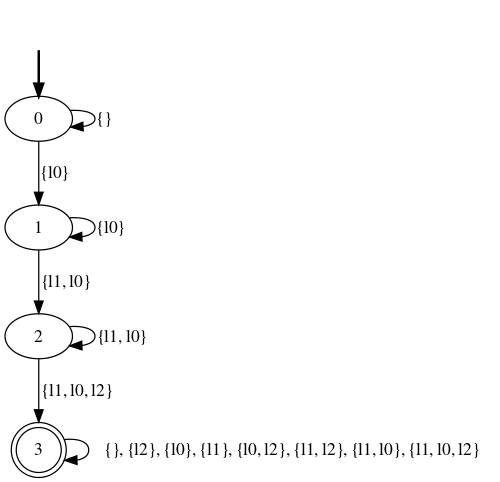
\includegraphics[width=0.6\textwidth]{images/breakout.png}
 	\caption{The automaton associated to the \LDLf formula in Equation \ref{eq:breakout-temporal-goal} for \Breakout 3x3.}
 	\label{fig:breakout-automaton}
\end{figure}

The features for fluents evaluation, for every temporal goal, are the status of each brick (present or removed). Recalling the notation used in Example \ref{exa:breakout}: $\tup{b_{11}, \dots, b_{nm}}$.

It is crucial to remark that the evaluation of the fluent from the features is different among the temporal goals above mentioned, despite the formulas are structurally the same (apart from the number of lines to remove). Indeed, thanks to the fluents evaluation phase (i.e. the map from features values to truth of each fluent), the formulas behave differently.

\paragraph{Configurations:}
The reinforcement algorithm used is Sarsa$(\lambda)$ (e.g. Sarsa with eligibility traces) with $\epsilon$-greedy policy. The values of the parameters are:
\begin{itemize}
	 \item $\lambda = 0.99$
	 \item $\DiscFact=0.999$	
	 \item $\alpha=0.1$
	 \item $\epsilon= 0.1$
\end{itemize}

The experiments are stopped when in the last 100 episodes of optimal runs the agent always achieved both the environment goal and the temporal goals.
Notice that this approach may yield a sub-optimal policy, but the found policies always satisfy \LLf goals.

\subsection{Optimal policies}
Now we show some screenshots of the optimal policies found for some of the temporal goals described before. You can find full recordings at \url{https://www.youtube.com/channel/UChpe0QEtRSKh4uCy5f2XuGA}.

\subsubsection{\textsc{Break-Cols-LR}}
In Figure \ref{exa:breakout-33-lr} are depicted the highlights of a run of the optimal policy for the goal \textsc{Break-Cols-LR}. As you can notice, the constraint expressed by the formula in Equation \ref{eq:breakout-temporal-goal} is satisfied (i.e. the columns of bricks are broken from left to right).

\begin{figure}[h]
	\centering
	\begin{subfigure}[b]{0.23\textwidth}
		
\includegraphics[width=\textwidth]{images/breakout-33-lr-1.png}
		%	 	\caption{a}
		%	 	\label{a}
	\end{subfigure}
	~ %add desired spacing between images, e. g. ~, \quad, \qquad, \hfill etc. 
	%(or a blank line to force the subfigure onto a new line)
	\begin{subfigure}[b]{0.23\textwidth}
		
\includegraphics[width=\textwidth]{images/breakout-33-lr-2bis.png}
		%	 	\caption{}
		%	 	\label{}
	\end{subfigure}
	~ %add desired spacing between images, e. g. ~, \quad, \qquad, \hfill etc. 
	%(or a blank line to force the subfigure onto a new line)
	\begin{subfigure}[b]{0.23\textwidth}
		
\includegraphics[width=\textwidth]{images/breakout-33-lr-2.png}
		%	 	\caption{}
		%	 	\label{}
	\end{subfigure}
	\begin{subfigure}[b]{0.23\textwidth}
		
\includegraphics[width=\textwidth]{images/breakout-33-lr-3.png}
		%	 	\caption{}
		%	 	\label{}
	\end{subfigure}
	\caption{A run of the learnt optimal policy for the task \textsc{Break-Cols-LR}. From left to right, you can see that the columns are broken in the right order.}\label{exa:breakout-33-lr}
\end{figure}

\subsubsection{\textsc{Break-Cols-BT}}
In Figure \ref{exa:breakout-33-bt} are depicted the highlights of a run of the optimal policy for the goal \textsc{Break-Cols-BT}. The constraint expressed by the formula in Equation \ref{eq:breakout-temporal-goal} is satisfied (i.e. the rows of bricks are broken from the bottom to the top).


\begin{figure}[h]
	\centering
	\begin{subfigure}[b]{0.23\textwidth}
		
\includegraphics[width=\textwidth]{images/breakout-33-bt-1.png}
		%	 	\caption{a}
		%	 	\label{a}
	\end{subfigure}
	~ %add desired spacing between images, e. g. ~, \quad, \qquad, \hfill etc. 
	%(or a blank line to force the subfigure onto a new line)
	\begin{subfigure}[b]{0.23\textwidth}
		
\includegraphics[width=\textwidth]{images/breakout-33-bt-2bis.png}
		%	 	\caption{}
		%	 	\label{}
	\end{subfigure}
	~ %add desired spacing between images, e. g. ~, \quad, \qquad, \hfill etc. 
	%(or a blank line to force the subfigure onto a new line)
	\begin{subfigure}[b]{0.23\textwidth}
		
\includegraphics[width=\textwidth]{images/breakout-33-bt-2.png}
		%	 	\caption{}
		%	 	\label{}
	\end{subfigure}
	\begin{subfigure}[b]{0.23\textwidth}
		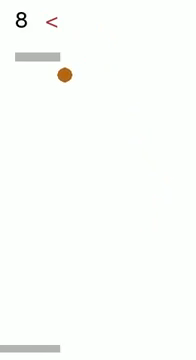
\includegraphics[width=\textwidth]{images/breakout-33-bt-3.png}
		%	 	\caption{}
		%	 	\label{}
	\end{subfigure}
	\caption{A run of the learnt optimal policy for the task \textsc{Break-Cols-LR}. From the bottom to the top, you can see that the rows are broken in the right order.}\label{exa:breakout-33-bt}
\end{figure}


\subsubsection{\textsc{Break-Cols-RL-TB}}
In Figure \ref{exa:breakout-33-rl-tb} are depicted the highlights of a run of the optimal policy for the goal \textsc{Break-Cols-RL-TB}. Notice that, even in the case of multiple temporal goal, the constraints expressed by the formula in Equation \ref{eq:breakout-temporal-goal} are satisfied (i.e. the rows of bricks are broken from the top to the bottom and the columns of bricks are broken from right to left). Furthermore, notice that the formula is the same, but \emph{how the fluents are evaluated from the features}  makes the difference.


\begin{figure}[h]
	\centering
	\begin{subfigure}[b]{0.18\textwidth}
		
\includegraphics[width=\textwidth]{images/breakout-33-rl-tb-1.png}
		%	 	\caption{a}
		%	 	\label{a}
	\end{subfigure}
	~ %add desired spacing between images, e. g. ~, \quad, \qquad, \hfill etc. 
	%(or a blank line to force the subfigure onto a new line)
	\begin{subfigure}[b]{0.18\textwidth}
		
\includegraphics[width=\textwidth]{images/breakout-33-rl-tb-2.png}
		%	 	\caption{}
		%	 	\label{}
	\end{subfigure}
	~ %add desired spacing between images, e. g. ~, \quad, \qquad, \hfill etc. 
	%(or a blank line to force the subfigure onto a new line)
	\begin{subfigure}[b]{0.18\textwidth}
		
\includegraphics[width=\textwidth]{images/breakout-33-rl-tb-3.png}
		%	 	\caption{}
		%	 	\label{}
	\end{subfigure}
	\begin{subfigure}[b]{0.18\textwidth}
		
\includegraphics[width=\textwidth]{images/breakout-33-rl-tb-4.png}
		%	 	\caption{}
		%	 	\label{}
	\end{subfigure}
	\begin{subfigure}[b]{0.18\textwidth}
		
\includegraphics[width=\textwidth]{images/breakout-33-rl-tb-5.png}
		%	 	\caption{}
		%	 	\label{}
	\end{subfigure}
	\caption{A run of the learnt optimal policy for the task \textsc{Break-Cols-LR}. From the bottom to the top, you can see that the rows are broken in the right order.}\label{exa:breakout-33-rl-tb}
\end{figure}

\subsection{Benchmarking of reward shaping techniques}
In this section we report some statistics about the performances of the proposed approach with a focus on automata-based reward shaping.
For each configuration we collected the observed reward for each episode, over 10 runs. Each run has a time limit of 10000 episodes.
Then we moving averaged the sequences of rewards with a window of size 100, in order to make the curves more smoothed, and averaged the result across all the runs. The plots show this processed sequences  over the number of episodes. The colored bands represents the 90\% confidence interval taken from bootstrapped re-samples.

We show our results in two parts:
\begin{enumerate}
	\item Comparison of \emph{No Reward Shaping}, \emph{Off-line Reward Shaping} and \emph{On-the-fly Reward Shaping} in \Breakout 3x3, 3x4 and 4x4, with temporal goal \textsc{Break-Cols-LR};
	\item Comparison of \emph{No Reward Shaping}, \emph{Off-line Reward Shaping} and \emph{On-the-fly Reward Shaping} in Breakout 4x4, with temporal goals \textsc{Break-Cols-LR}, \textsc{Break-Rows-BT}, \textsc{Break-Cols-LR \& Break-Rows-BT};
\end{enumerate}

\subsubsection{Different number of bricks and rows}
In Figure \ref{fig:breakout-benchmarking-reward-shaping-lr-different-bricks} are plotted different statistics by increasing difficulty in the environment, for every variant of reward shaping technique.
On the x-axis the number of episodes, on the y-axis the average reward (obtained as explained above). In every case, we can see that the use of reward shaping (both off-line and on-the-fly) speed-up the learning process.
\begin{figure}[h]
	 \centering
	 \begin{subfigure}[b]{0.65\textwidth}
	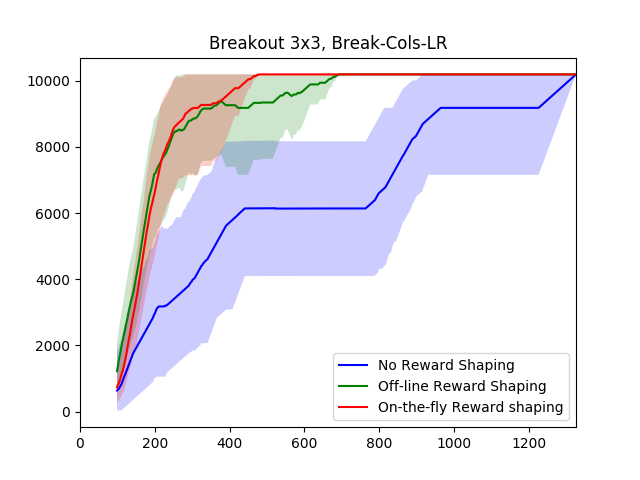
\includegraphics[width=\textwidth]{images/rs-comparison_b33.png}
	 	\caption{\Breakout 3x3, \textsc{Break-Cols-LR} for three different settings: \emph{No RS}, \emph{Off-line RS} and \emph{On-the-fly RS}}
	 	\label{fig:breakout-benchmarking-reward-shaping-33-lr}
	 \end{subfigure}
	 ~ %add desired spacing between images, e. g. ~, \quad, \qquad, \hfill etc. 
	 %(or a blank line to force the subfigure onto a new line)
	 \begin{subfigure}[b]{0.65\textwidth}
		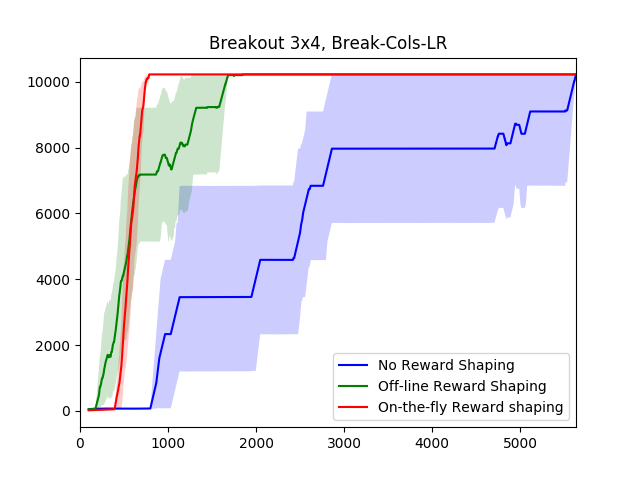
\includegraphics[width=\textwidth]{images/rs-comparison_b34.png}
	 	\caption{\Breakout 3x4, \textsc{Break-Cols-LR} for three different settings: \emph{No RS}, \emph{Off-line RS} and \emph{On-the-fly RS}}
	 	\label{fig:breakout-benchmarking-reward-shaping-34-lr}
	 \end{subfigure}
	 ~ %add desired spacing between images, e. g. ~, \quad, \qquad, \hfill etc. 
	 %(or a blank line to force the subfigure onto a new line)
	 \begin{subfigure}[b]{0.65\textwidth}
	 	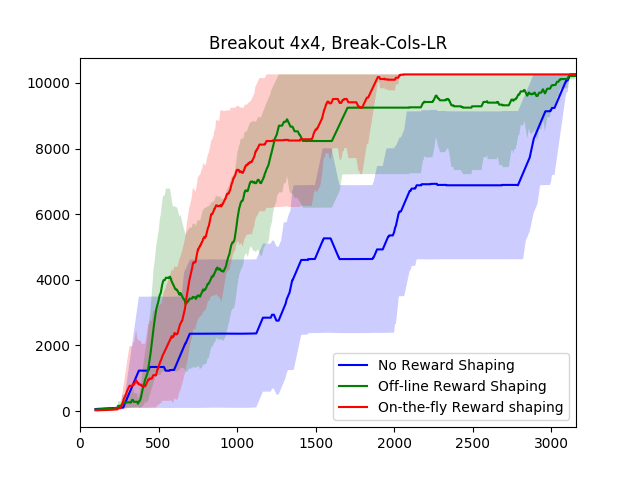
\includegraphics[width=\textwidth]{images/rs-comparison_b44.png}
	 	\caption{\Breakout 4x4, \textsc{Break-Cols-LR} for three different settings: \emph{No RS}, \emph{Off-line RS} and \emph{On-the-fly RS}}
	 	\label{fig:breakout-benchmarking-reward-shaping-44-lr}
	 \end{subfigure}
	 \caption{The results of three settings are reported, namely: \Breakout 3x3, 3x4 and 4x4 (\ref{fig:breakout-benchmarking-reward-shaping-33-lr}, \ref{fig:breakout-benchmarking-reward-shaping-34-lr} and  \ref{fig:breakout-benchmarking-reward-shaping-44-lr} respectively), all of them with temporal goal \textsc{Break-Cols-LR}. In every case, we can see that the use of reward shaping (both off-line and on-the-fly) speed-up the learning process. }\label{fig:breakout-benchmarking-reward-shaping-lr-different-bricks}
\end{figure}


\subsubsection{Different temporal goals}
In Figure \ref{fig:breakout-benchmarking-reward-shaping-44-different-goal} Here we show the performances by varying the temporal goals.
On the x-axis the number of episodes, on the y-axis the average reward (obtained as explained above). In every case, we can see that the use of reward shaping (both off-line and on-the-fly) speed-up the learning process.
\begin{figure}[h]
	\centering
	\begin{subfigure}[b]{0.65\textwidth}
		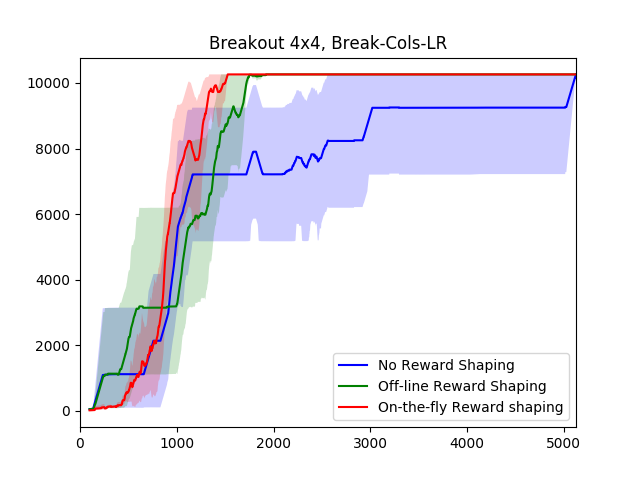
\includegraphics[width=\textwidth]{images/b44-cols-comparison}
	 	\caption{\Breakout 4x4, \textsc{Break-Cols-LR} for three different settings: \emph{No RS}, \emph{Off-line RS} and \emph{On-the-fly RS}}
		\label{fig:breakout-benchmarking-reward-shaping-44-lr-varying-goal}
	\end{subfigure}
	~ %add desired spacing between images, e. g. ~, \quad, \qquad, \hfill etc. 
	%(or a blank line to force the subfigure onto a new line)
	\begin{subfigure}[b]{0.65\textwidth}
		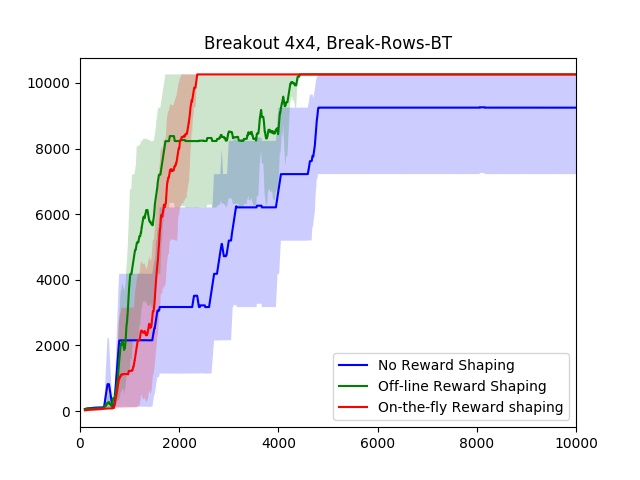
\includegraphics[width=\textwidth]{images/b44-rows-comparison}
	 	\caption{\Breakout 4x4, \textsc{Break-Rows-BT} for three different settings: \emph{No RS}, \emph{Off-line RS} and \emph{On-the-fly RS}}
		\label{fig:breakout-benchmarking-reward-shaping-44-bt-varying-goal}
	\end{subfigure}
	~ %add desired spacing between images, e. g. ~, \quad, \qquad, \hfill etc. 
	%(or a blank line to force the subfigure onto a new line)
	\begin{subfigure}[b]{0.65\textwidth}
		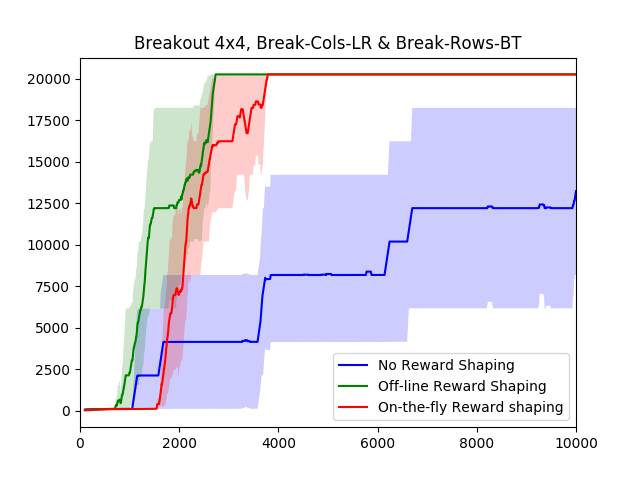
\includegraphics[width=\textwidth]{images/b44-both-comparison}
		\caption{\Breakout 4x4, \textsc{Break-Cols-LR \& Break-Rows-LR} for three different settings: \emph{No RS}, \emph{Off-line RS} and \emph{On-the-fly RS}}
		\label{fig:breakout-benchmarking-reward-shaping-44-lr-bt-varying-goal}
	\end{subfigure}
	\caption{The results of three settings are reported, namely: \Breakout 4x4 with temporal goal \textsc{Break-Cols-LR}, \textsc{Break-Cols-BT} and \textsc{Break-Cols-LR \& \textsc{Break-Cols-BT}} (\ref{fig:breakout-benchmarking-reward-shaping-44-lr-varying-goal}, \ref{fig:breakout-benchmarking-reward-shaping-44-bt-varying-goal} and  \ref{fig:breakout-benchmarking-reward-shaping-44-lr-bt-varying-goal} respectively). In every case, we can see that the use of reward shaping (both off-line and on-the-fly) speed-up the learning process. }\label{fig:breakout-benchmarking-reward-shaping-44-different-goal}
\end{figure}

\section{\Sapientino}
TODO
\section{\Minecraft}
TODO